    \begin{center}
\renewcommand{\arraystretch}{1.5}
$
\begin{array}{r r r r c r | l}
    % Riga 1: Dividendo e Divisore
    p^6 & \hspace{8mm} & + p^4 & + p^3 & \hspace{8mm} & \hspace{8mm} & p^3 + p^2 + 1 \\ 
    \cline{7-7}
    % Riga 2: Quoziente
        &        &       &       &       &       & p^3 + p^2 \\ 
    \cline{1-6}
    % Riga 3: Passaggi intermedi
    p^6 & + p^5  &       & + p^3 &       &       & \\ 
        & + p^5  & + p^4 & + p^3 &       &       & \\ 
    \cline{1-6}
    % Riga 5: Termine da cerchiare (Centrato nella colonna 5)
        & + p^5  & + p^4 &       & + p^2 &       & \\ 
    \cline{1-6}
    % Riga 6: Resto cerchiato (Allineato perfettamente grazie al 'c' della colonna)
        &        &       &       & 
            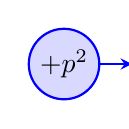
\begin{tikzpicture}[baseline=(R.base)]
                \node[draw=blue, fill=blue!15, circle, inner sep=2pt, thick] (R) {$+ p^2$};
                % L'overlay evita che la freccia sposti il cerchio a sinistra
                \draw[blue, thick, ->, >=stealth, overlay] (R.east) -- ++(0.4,0) node[right] {R(p)};
            \end{tikzpicture}
        & & 
\end{array}
$
\end{center}